%%%%%%%%%%%%%%%%%%%%%%%%%%%%%%%%%%%%%%%%%%%%%%%%%%%%%%%%%%%%%%%%%%%%%%%%%%
% File: Lecture_1.tex
% Authors: James Kress
% Date: February 1, 2014
% Description: 
%%%%%%%%%%%%%%%%%%%%%%%%%%%%%%%%%%%%%%%%%%%%%%%%%%%%%%%%%%%%%%%%%%%%%%%%%%

%<<<<<<<<<<<<<<<<<<<<<<<<<<<<<<<<<<<<<<<<<<<<<<<<<<<<<<<<<<<<<<<<<<<<<<<<<<<<<%
% Document package information
%>>>>>>>>>>>>>>>>>>>>>>>>>>>>>>>>>>>>>>>>>>>>>>>>>>>>>>>>>>>>>>>>>>>>>>>>>>>>>%
\documentclass[xcolor=dvipsnames]{beamer} 
%%%%%%%%%%%%%%%%%%%%%%%%%%%%%%%%%%%%%%%%%%%%%%%%%%%%%%%%%%%%%%%%%%%%%%%%%%
% File: _TeXdefs.tex
% Author: James Kress
% Date: January 25, 2014
% Description: A tex file containing the \usepackage declarations, and
%			   other document critial style settings.
%%%%%%%%%%%%%%%%%%%%%%%%%%%%%%%%%%%%%%%%%%%%%%%%%%%%%%%%%%%%%%%%%%%%%%%%%%

%-----------Package imports
\usepackage{graphicx}
\usepackage{pgfpages}
\usepackage{tikz}
\usepackage{latexsym}
\usepackage{verbatim}
%//////////END package imports


%----------Style elements
\useoutertheme{infolines} 
\usetheme{Frankfurt} 
\usepackage{../theme/beamercolorthemeoregon}
\setbeamertemplate{sections/subsections in toc}[default]
\setbeamertemplate{footline}
{
\leavevmode%
  \hbox{%
  \begin{beamercolorbox}[wd=.3\paperwidth,ht=2.25ex,dp=.75ex,center]{institute in head/foot}%
    \usebeamerfont{institute in head/foot}\insertshortinstitute
  \end{beamercolorbox}%
    \begin{beamercolorbox}[wd=.4\paperwidth,ht=2.25ex,dp=.75ex,center]{title in head/foot}%
      \usebeamerfont{title in head/foot}\insertshorttitle
    \end{beamercolorbox}%
  \begin{beamercolorbox}[wd=.3\paperwidth,ht=2.25ex,dp=.75ex,center]{date in head/foot}%
    \usebeamerfont{date in head/foot}\insertshortdate\hspace*{3em}
    \insertframenumber{} / \inserttotalframenumber\hspace*{1ex}
  \end{beamercolorbox}}%
  \vskip0pt%
}
%/////////END style elements


%---------Command Declarations
\DeclareGraphicsExtensions{.pdf, .jpeg, .png, .jpg}
\graphicspath{ {../images/} }
\newcommand{\className}{\text{CIS 410/510} \\ \text{Parallel Computing}}
\newcommand{\departmentName}{\textit{Department of Computer and 
									Information Science \\ University of Oregon}}
%/////////END command declarations


%---------Setup pdf properties
\hypersetup{
	pdfusetitle=true,
    bookmarks=true,         	% show bookmarks bar?
    unicode=false,          	% non-Latin characters in Acrobat’s bookmarks
    pdftoolbar=true,        	% show Acrobat’s toolbar?
    pdfmenubar=true,        	% show Acrobat’s menu?
    pdffitwindow=false,     	% window fit to page when opened
    pdfstartview={Fit},   		% fits the width of the page to the window    
    pdfauthor={},     % author
    pdfsubject={Parallel Programming},   	% subject of the document
    pdfcreator={},   			% creator of the document
    pdfproducer={}, 			% producer of the document
    pdfkeywords={University of Oregon, parallel programming}, 
    pdfnewwindow=true,      	% links in new window
    colorlinks=true,       		% false: boxed links; true: colored links
    linkcolor=white,          	% color of internal links
    hidelinks,
    citecolor=green,        	% color of links to bibliography
    filecolor=magenta,      	% color of file links
    urlcolor=cyan,           	% color of external links
    linktoc=page,
    pageanchor = true
}
%//////////END setup pdf properties


%END ALL


\setbeamertemplate{caption}{\insertcaption}
%<<<<<<<<<<<<<<<<<<<<<<<<<<<<<<<<<<<<<<<<<<<<<<<<<<<<<<<<<<<<<<<<<<<<<<<<<<<<<%
% END Document package information
%>>>>>>>>>>>>>>>>>>>>>>>>>>>>>>>>>>>>>>>>>>>>>>>>>>>>>>>>>>>>>>>>>>>>>>>>>>>>>%

%=============================================================================%
% Begining: Title Page Material
%=============================================================================%
\begin{document}
	\title[Pipeline Pattern]{Pipeline Pattern}
	\author[]{\className}
	\institute[\className]{\departmentName}
	\date{} 

	\titlegraphic{\centering 
		$\vcenter{\hbox{
\includegraphics[height=.31in,width=2.0in]{oregonLogo}}}$
	}

	\begin{frame}
		\maketitle
	\end{frame}
	
	\section{Introduction} 
		\subsection{} 
			\begin{frame}{Developer Training}
				\begin{center}
					\vspace{-.5in} 
\includegraphics[width=0.4\textwidth]{images/OSNAP_logo} 
					
					Pipeline Pattern
					
					Extraterrestrial Message Recovery
				\end{center}
			\end{frame}
			
			\begin{frame}{Extraterrestrial Message Recovery}
				\begin{columns}
					\begin{column}{0.5\textwidth}
							O-SNAP routinely monitors space for alien messages. \newline
							
							Recently, a message was intercepted, and management needs it decoded. The message suffered degradation during its journey so a series of transformations will need to be applied to recover the original message. 
					\end{column}
					\begin{column}{0.5\textwidth}
						
\includegraphics[width=\textwidth]{images/alteredVideoFrame}
					\end{column}
				\end{columns}
			\end{frame}
		
		
	\section{Damage Suffered to Video} 
		\subsection{} 
			\begin{frame}{Damage Suffered to Video}
				The damage that was suffered by the video is known, as is the order that the damage occurred:
				\begin{itemize}
					\item Brightness was increased by 100 units
					\item Contrast was increased by a factor of 1.025x
					\item Each frame was rotated 20 degrees
					\item The pixels gbr (as read in opencv) value order was rearranged to be rgb, and the pixel was stored with a $y$ offset of 375 pixels and a $x$ offset of 475 pixels.
				\end{itemize}
			\end{frame}
			
			\begin{frame}{Basic Solution}
				Since the frame rotation and pixel rearrangement occurred in a specific order during the damage to the message, they need to be reversed in the right order or else the pixels will not be returned to the correct locations (See Figure), therefore, the stages for reconstruction will be:
				
				\begin{columns}
					\begin{column}{0.6\textwidth}
						\begin{itemize}
							\item Perform inverse of brightness increase
							\item Perform inverse of contrast increase
							\item Perform inverse of pixel reorder and rgb value rearrangement
							\item Perform inverse of frame rotation
						\end{itemize}
					\end{column}
					\begin{column}{0.40\textwidth}
						\vspace{-.25in}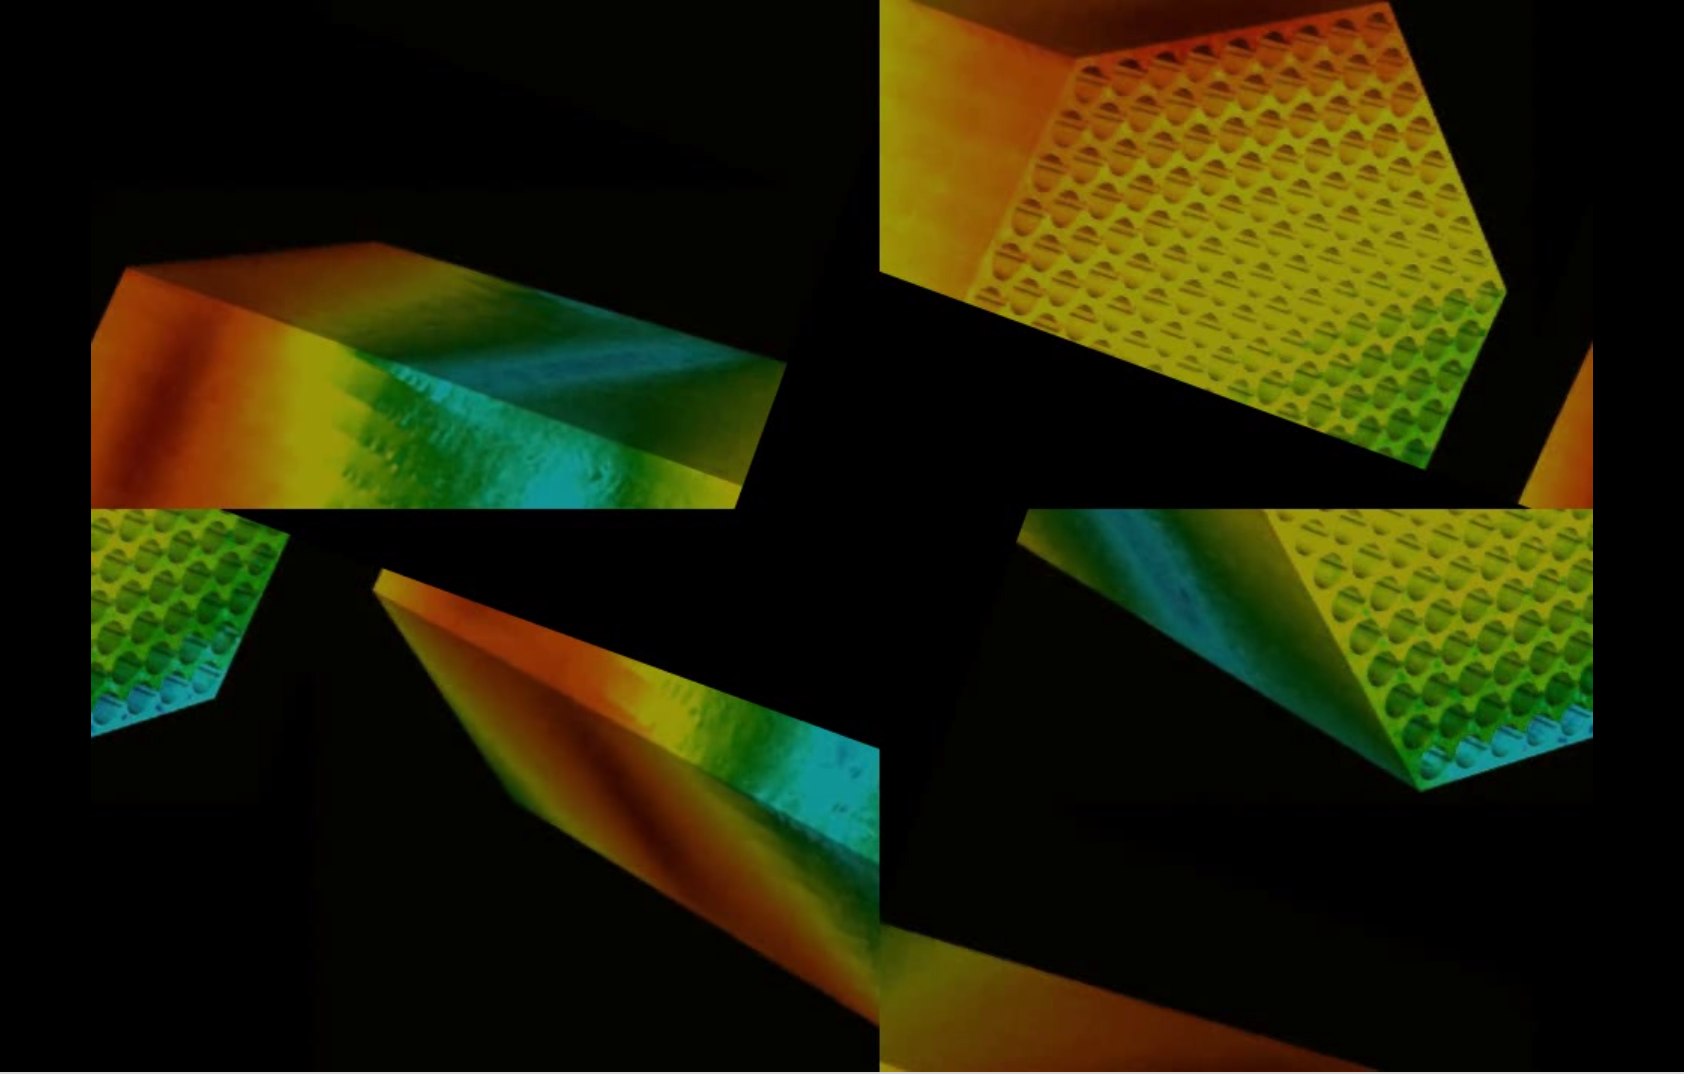
\includegraphics[width=\textwidth]{images/badPixels} 
					\end{column} 
				\end{columns}
				
			\end{frame}

	
	\section{Pattern}
		\subsection{} 
		  \begin{frame}{Pipeline Pattern}
				\begin{columns}
					\begin{column}{0.65\textwidth}
						\begin{itemize}
							\item Basic pipeline consists of a linear sequence of stages
							\item Connects tasks in a producer-consumer relationship
							\item Early items can flow all the way though the pipeline before later items become available 
							\item Can process large amounts of data using a fixed amount of memory
						\end{itemize}
					\end{column}
					\begin{column}{0.35\textwidth}
						\centering 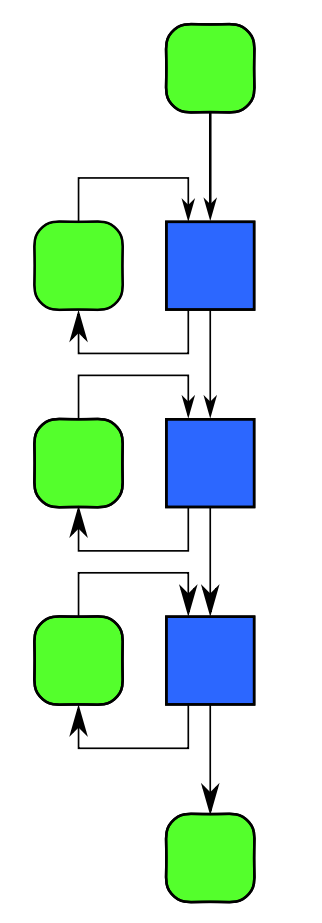
\includegraphics[width=1.in]{images/pipelinePattern}
					\end{column}
				\end{columns}
			\end{frame}
		
	
	\section{Parallel Approach}
		\subsection{} 
			\begin{frame}{What Our Pipeline Looks Like}
				The pipeline in this program consists of six individual stages:
				\begin{columns}
					\begin{column}{0.35\textwidth}
						\begin{enumerate}
							\item Read frames in order
							\item Fix brightness
							\item Fix contrast
							\item Fix pixel location
							\item Fix rotation
							\item Save frames in order
						\end{enumerate}
					\end{column}
					\begin{column}{0.65\textwidth}
						\centering 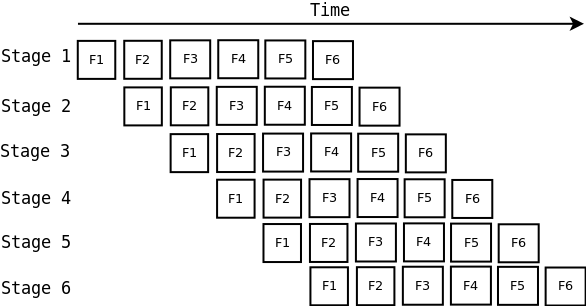
\includegraphics[width=2.9in]{images/pipelineDescDiagram}
					\end{column}
				\end{columns}	
			\end{frame}
			
			
			\begin{frame}{TBB Pipeline Constructs}
				TBB has a \textit{parallel\_pipeline} template:
				\begin{itemize}[<+->]
					\item Construct a \textit{filter\_t$<$X, Y$>$} for each stage
						\begin{itemize}
							\item First stage must have type \textit{filter\_t$<$void, ...$>$}
							\item Last stage must have type \textit{filter\_t$<$..., void$>$}
						\end{itemize}
					\item Glue the stages together with \textit{operator\&}
						\begin{itemize}
							\item Top level glued result must be a \textit{filter\_t$<$void, void$>$}
						\end{itemize}
					\item Invoke \textit{parallel\_pipeline} on the \textit{filter\_t$<$void, void$>$}
				\end{itemize}
			\end{frame} 
	
	
	\section{Examples} 
		\subsection{} 
			\begin{frame}{Serial Pipeline Example}
				A serial pipeline runs one data element completely though the pipeline before proceeding:
				\begin{columns}
					\begin{column}{0.35\textwidth}
						 There are three stages: \\ $f$, $g$, and $h$
					\end{column}
					\begin{column}{0.65\textwidth}
						\begin{figure}
							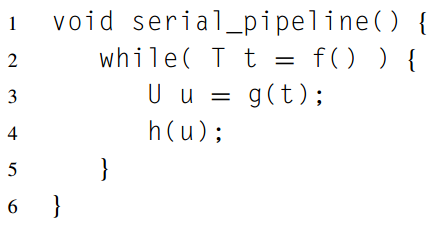
\includegraphics[width=2.in]{images/serialPipeline}
							\caption{LISTING 9.1}
						\end{figure} 
					\end{column}
				\end{columns}
				
			\end{frame}
		
		
			\begin{frame}{TBB Pipeline Example}
				\begin{columns}
					\begin{column}{0.45\textwidth}
						This pipeline runs in parallel:
							\begin{itemize}
								\item Stages $f$ and $h$ process one item and a time
								\item Stage $g$ processes multiple items in parallel
							\end{itemize} 
					\end{column}
					\begin{column}{0.55\textwidth}
						\begin{figure}
							\vspace{-.4in} 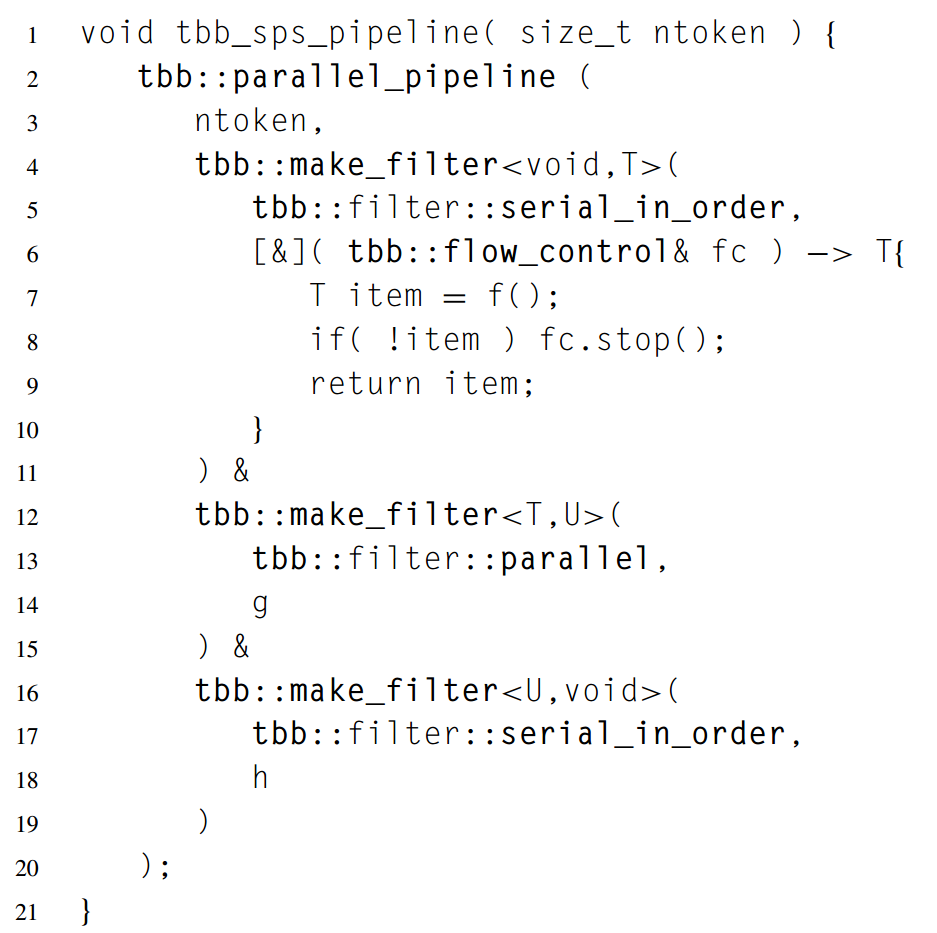
\includegraphics[width=2.65in]{images/parallelPipeline}
							\caption{LISTING 9.2}
						\end{figure} 
					\end{column}
				\end{columns}
			\end{frame}
		
		
	\section{Conclusion}
		  \begin{frame}{Key Points - Pipeline}
				\begin{itemize}
			      \item Concept: 
			      	\begin{itemize}
			      		\item Sequentially apply a series of operations on an data element
			      		\item All stages of the pipe can be active simultaneously
			      	\end{itemize}
			      \item Design:
			      	\begin{itemize}
			      		\item Challenge is ensuring operations do the same amount of work
			      	\end{itemize} 
			       \item Strengths:
			       \begin{itemize}
			       		\item Can process large amounts of data with fixed memory footprint
			       \end{itemize}
				 \item Weaknesses:
				 	\begin{itemize}
				 		\item Throughput limited to the throughput of slowest serial stage
				 		\item Addressable with parallel pipeline stages where possible
				 	\end{itemize}
				\end{itemize}
			\end{frame}


\end{document}
%END ALL

